\chapter{Estimating Feature Saliency Using 2D Saliency Maps \label{2d_saliency_map}}

\begin{figure}
	\centering
	\begin{minipage}{.33\textwidth}
		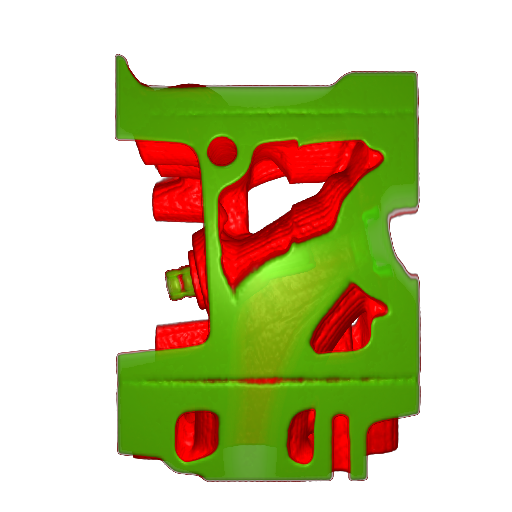
\includegraphics[width=1\linewidth]{images/engine_naive}
		\subcaption{}
	\end{minipage}~
	\begin{minipage}{.33\textwidth}
		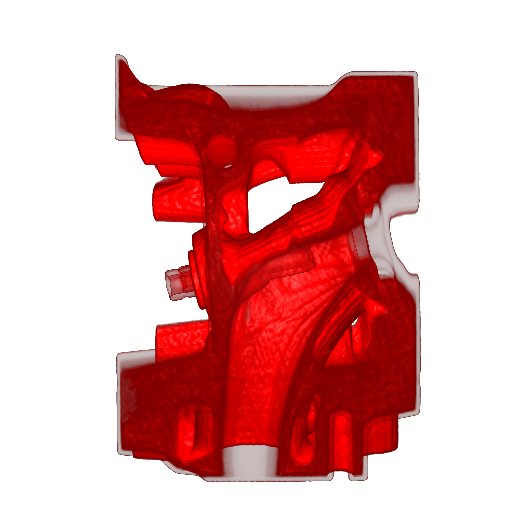
\includegraphics[width=1\linewidth]{images/engine_naive_1}
		\subcaption{}
	\end{minipage}~
	\begin{minipage}{.33\textwidth}
		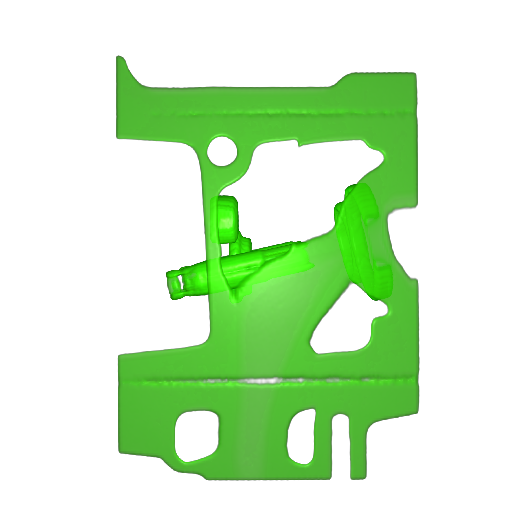
\includegraphics[width=1\linewidth]{images/engine_naive_2}
		\subcaption{}
	\end{minipage}
	\caption{Engine block and its features}
	\label{fig:engine_naive}
\end{figure}

\begin{figure}
	\centering
	\begin{minipage}{.33\textwidth}
		
\includegraphics[width=1\linewidth]{images/engine_naive_saliencemap}
		\subcaption{}
	\end{minipage}~
	\begin{minipage}{.33\textwidth}
		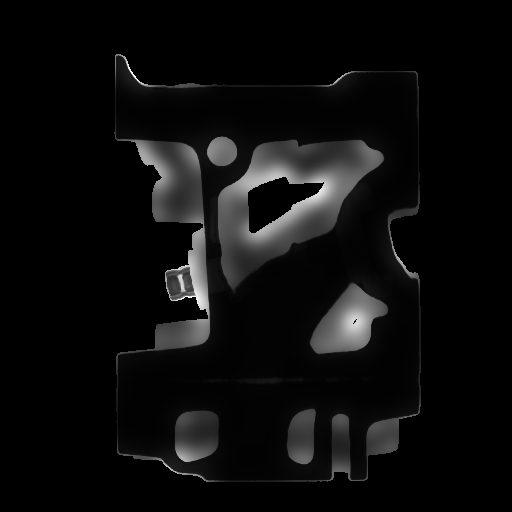
\includegraphics[width=1\linewidth]{images/engine_naive_saliencemap_1_overlap}
		\subcaption{}
	\end{minipage}~
	\begin{minipage}{.33\textwidth}
		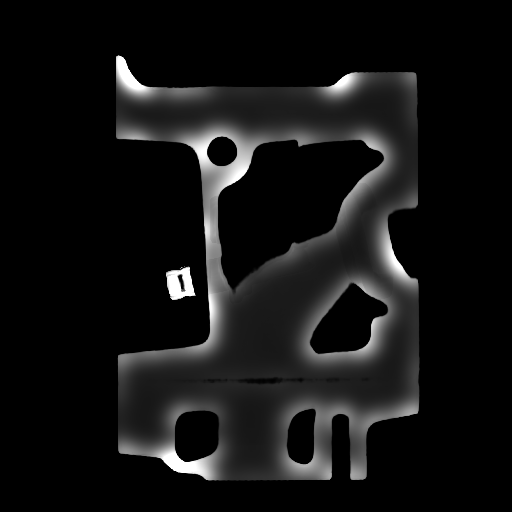
\includegraphics[width=1\linewidth]{images/engine_naive_saliencemap_2_overlap}
		\subcaption{}
	\end{minipage}
	\caption{2D saliency maps \cite{itti_model_1998}}
	\label{fig:engine_naive_saliencemap}
\end{figure}

\begin{figure}
	\centering
	\begin{minipage}{.33\textwidth}
		
\includegraphics[width=1\linewidth]{images/engine_naive_saliencemap_1}
		\subcaption{}
	\end{minipage}~
	\begin{minipage}{.33\textwidth}
		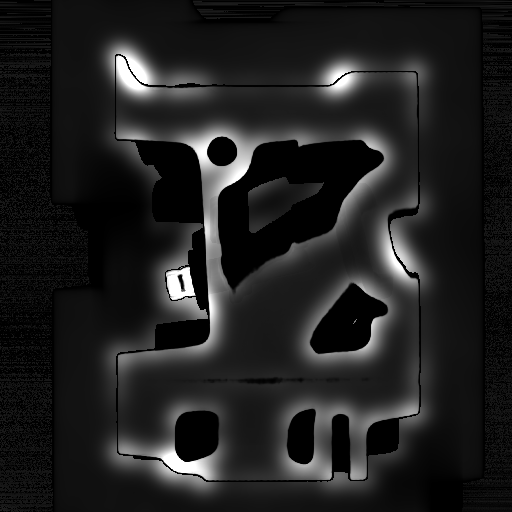
\includegraphics[width=1\linewidth]{images/engine_naive_saliencemap_2}
		\subcaption{}
	\end{minipage}
	\caption{feature saliency maps}
	\label{fig:engine_naive_saliencemap_features}
\end{figure}

